\section{Global Thermohaline circulation}
To get a better picture of the changes that occur during the time periods we compare differences in sea temperature at 250m depth. We do not use the sea surface temperature here because of the restoring boundary conditions used on the top layer of the ocean. Thus we can get a better idea of the transported temperature. First, we compare the temperature diffirence in the 55Ma basin and the 35Ma basin. We thus compare the temperature profiles of the late Paleocene to the late Eocene (\prettyref{fig:5535cooling}). Here we see substantial diffirences between the two. One of the key features of the Eocene seems to be a large amount of cooling in the southern Atlantic along with a heating in the southern pacific. Resulting from the large Increase in size of the southern subtropical gyre in the Indian ocean. 

\begin{figure}[H]
	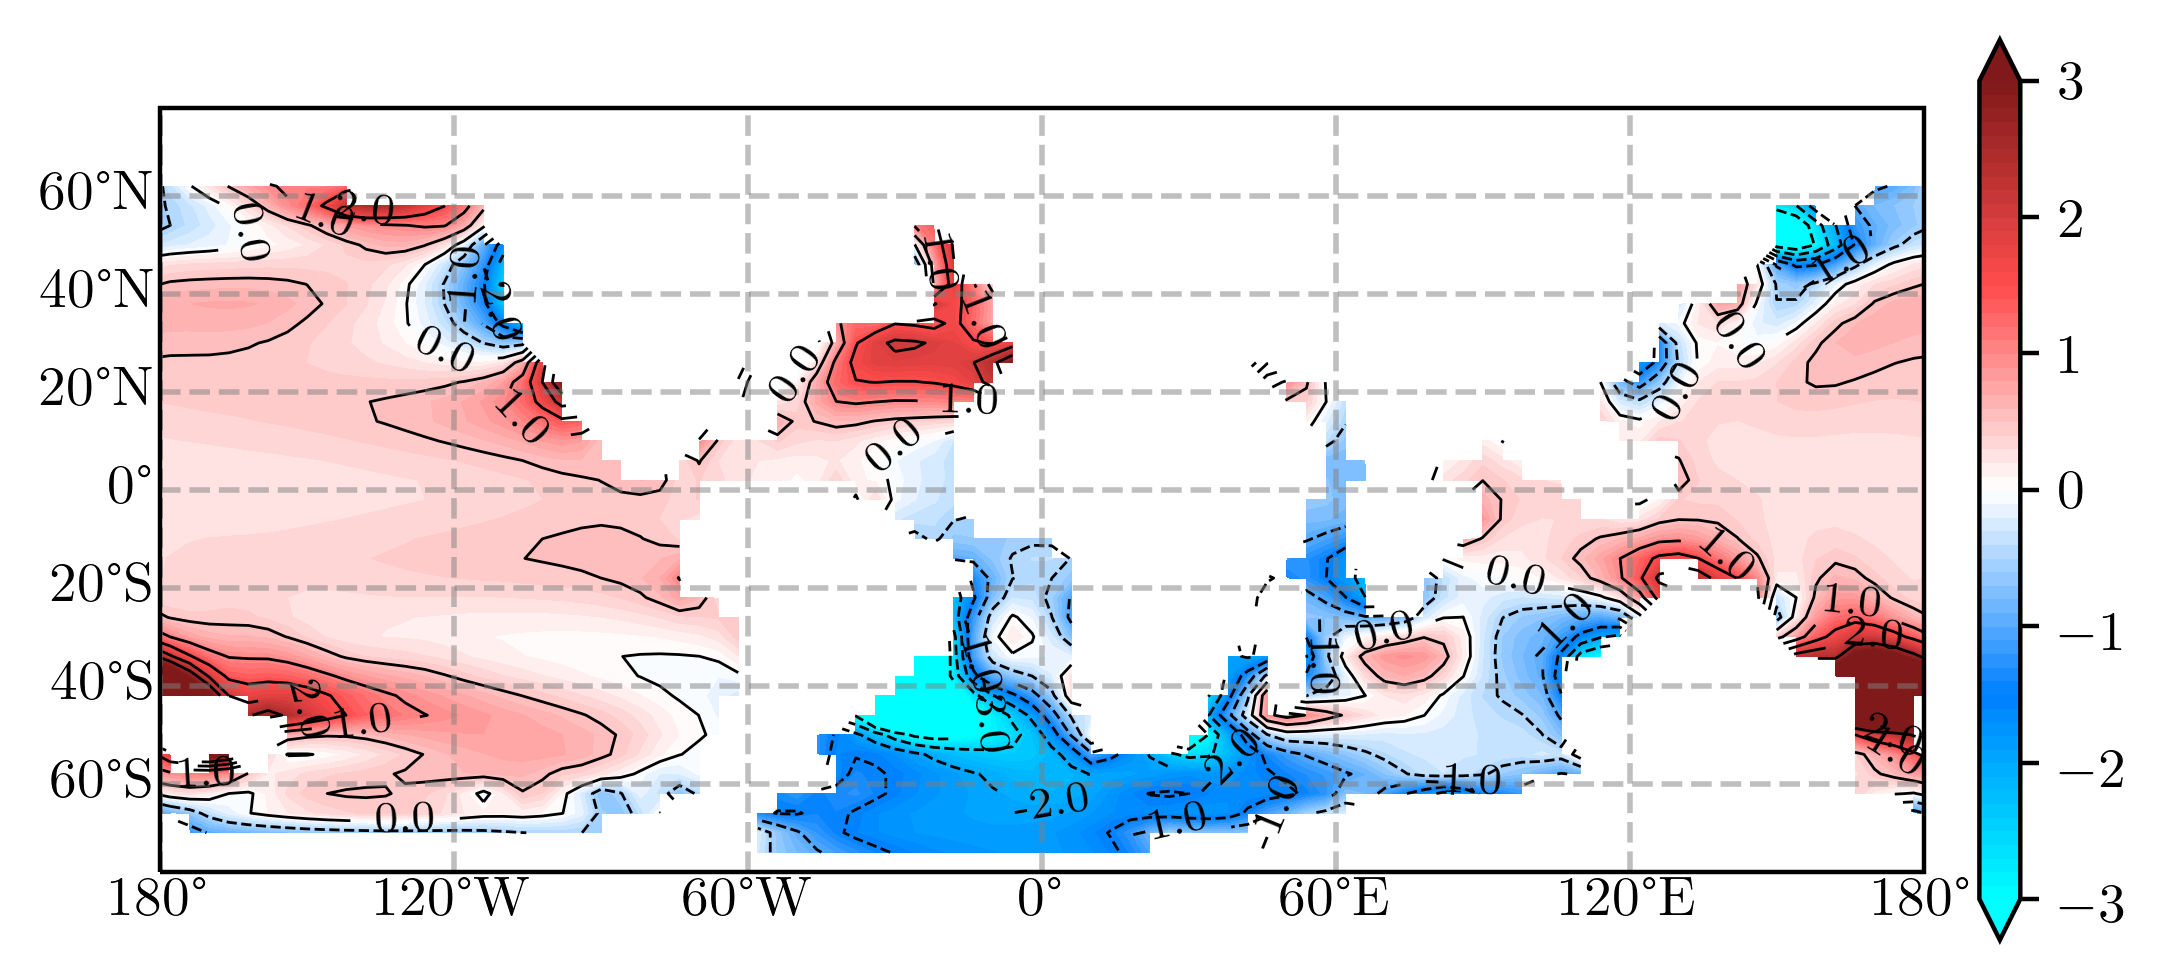
\includegraphics[width=\linewidth]{Paleo_eocene_55_35.png}
	\caption{Temperature diffirences between late Paleocene (55Ma) and late Eocene (35Ma) simulations. Positive values indicate warming, Negative values indicate cooling.}
	\label{fig:5535cooling}
\end{figure}

We also look at the changes between the late Eocene and the late Oligocene. 

\begin{figure}[H]
	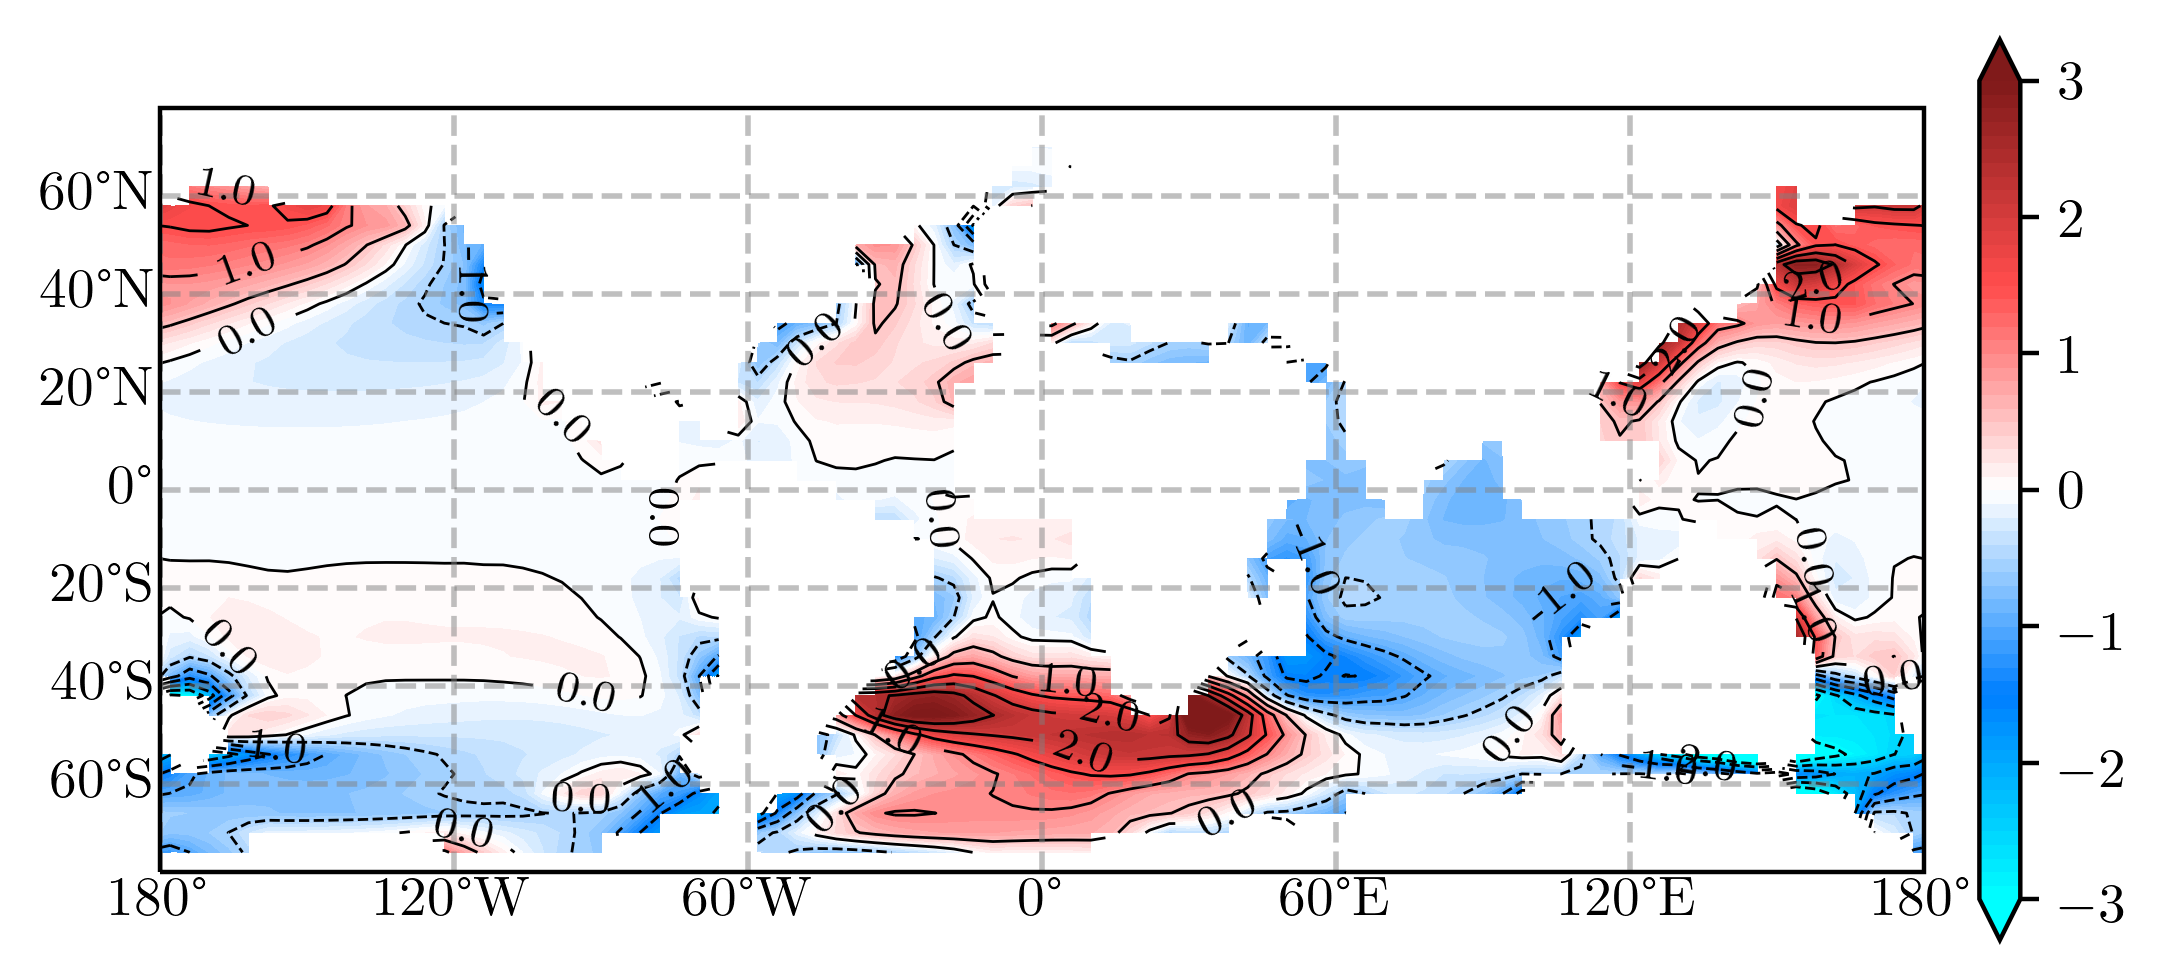
\includegraphics[width=\linewidth]{Paleo_eocene_35_20.png}
	\caption{Temperature diffirences between late Eocene (35Ma) and late Oligocene (20Ma) simulations. Positive values indicate warming, Negative values indicate cooling.}
	\label{fig:3520cooling}
\end{figure}

\begin{figure}[H]
	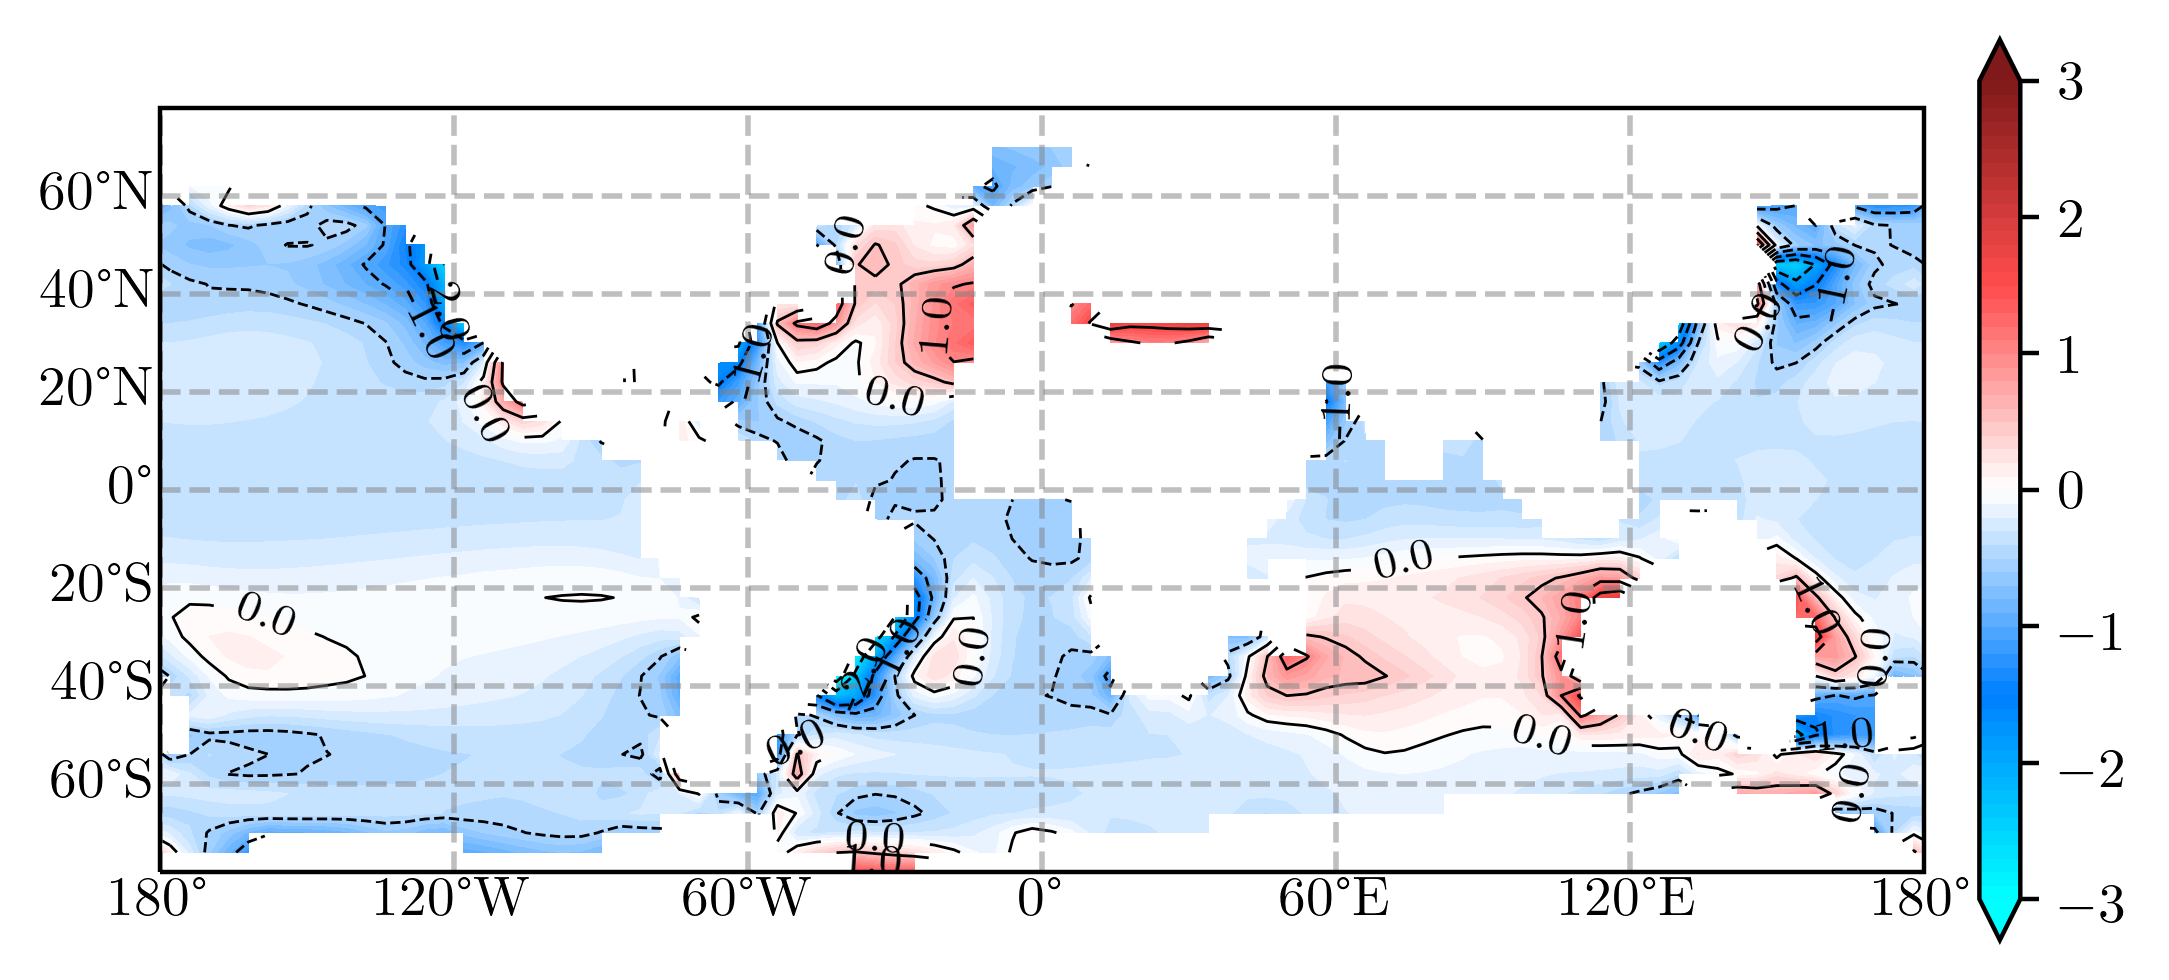
\includegraphics[width=\linewidth]{Paleo_eocene_20_10.png}
	\caption{Temperature diffirences between late Oligocene (20Ma) and middle Miocene (10Ma) simulations. Positive values indicate warming, Negative values indicate cooling.}
	\label{fig:2010cooling}
\end{figure}


\begin{figure}[H]
	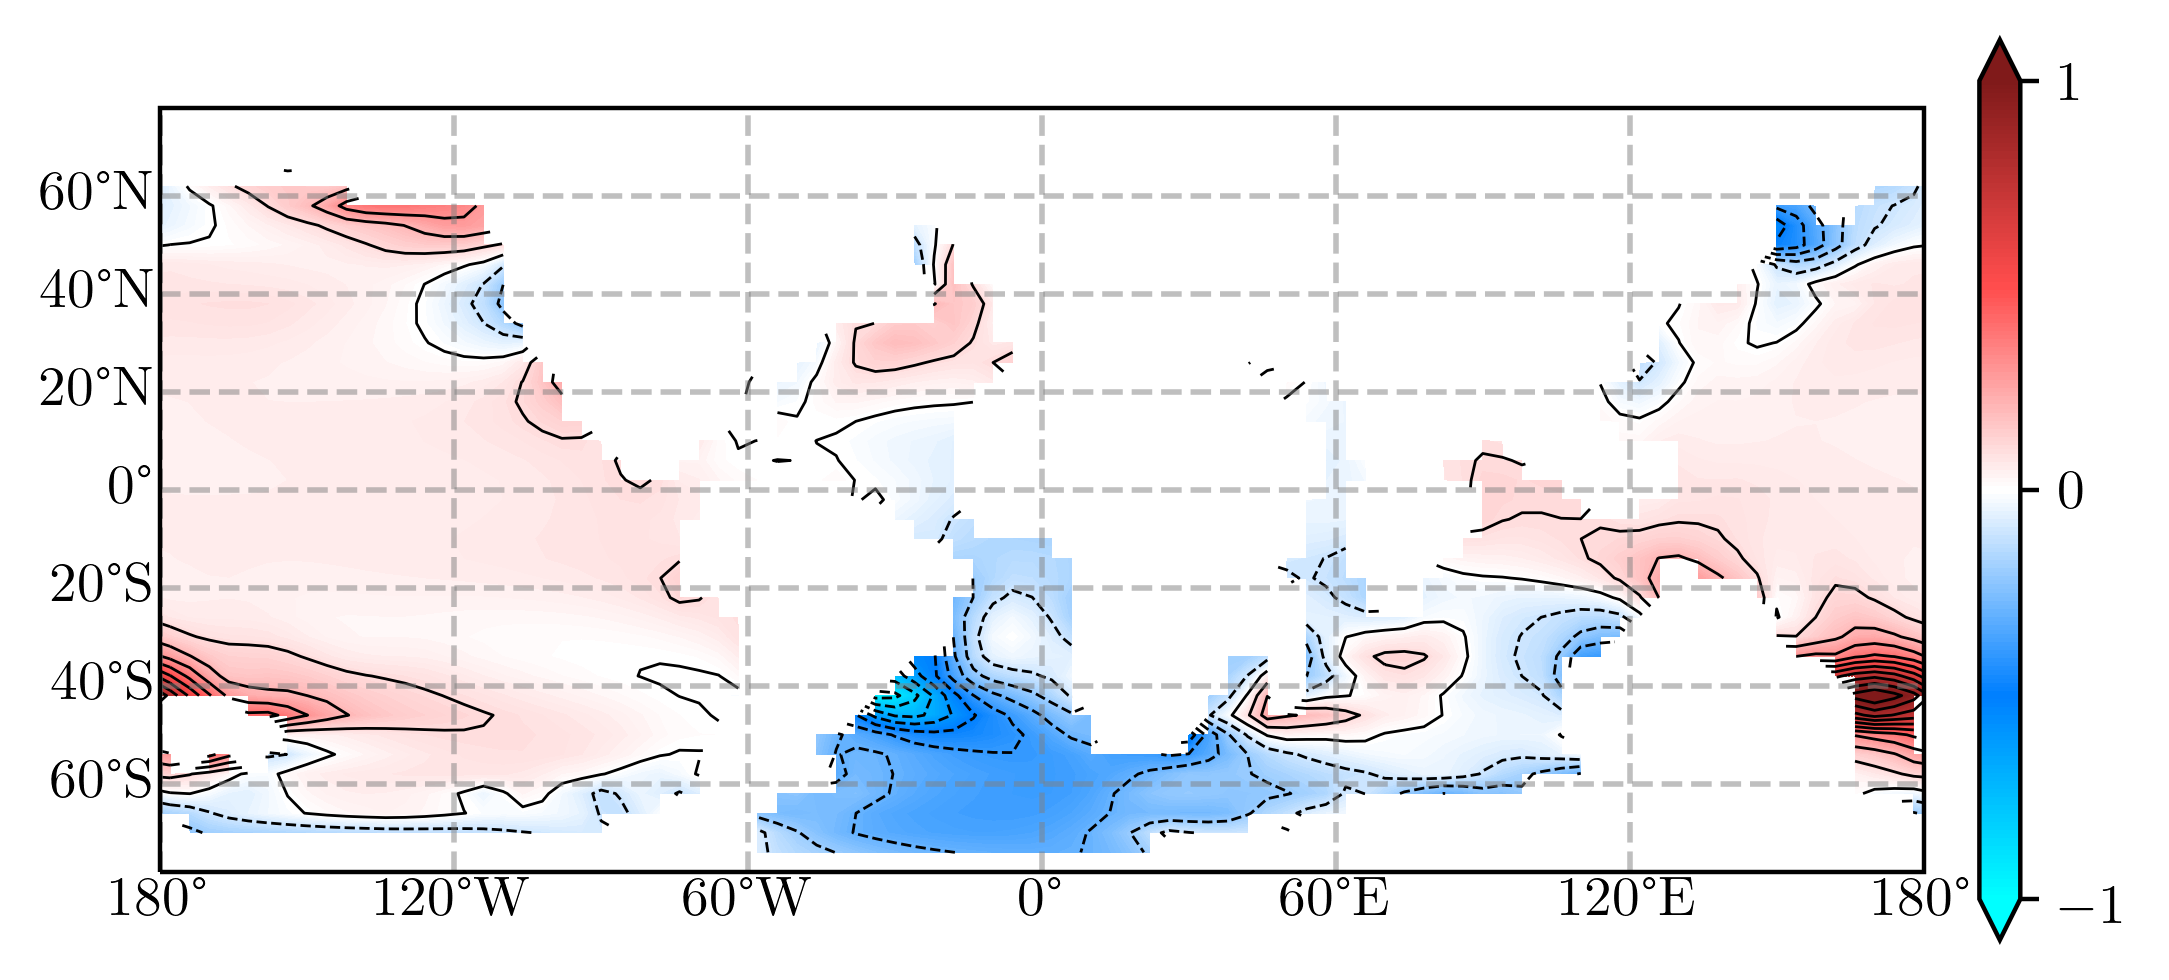
\includegraphics[width=\linewidth]{salt_55_35.png}
	\caption{SSS}
	\label{fig:salt5535cooling}
\end{figure}
\begin{figure}[H]
	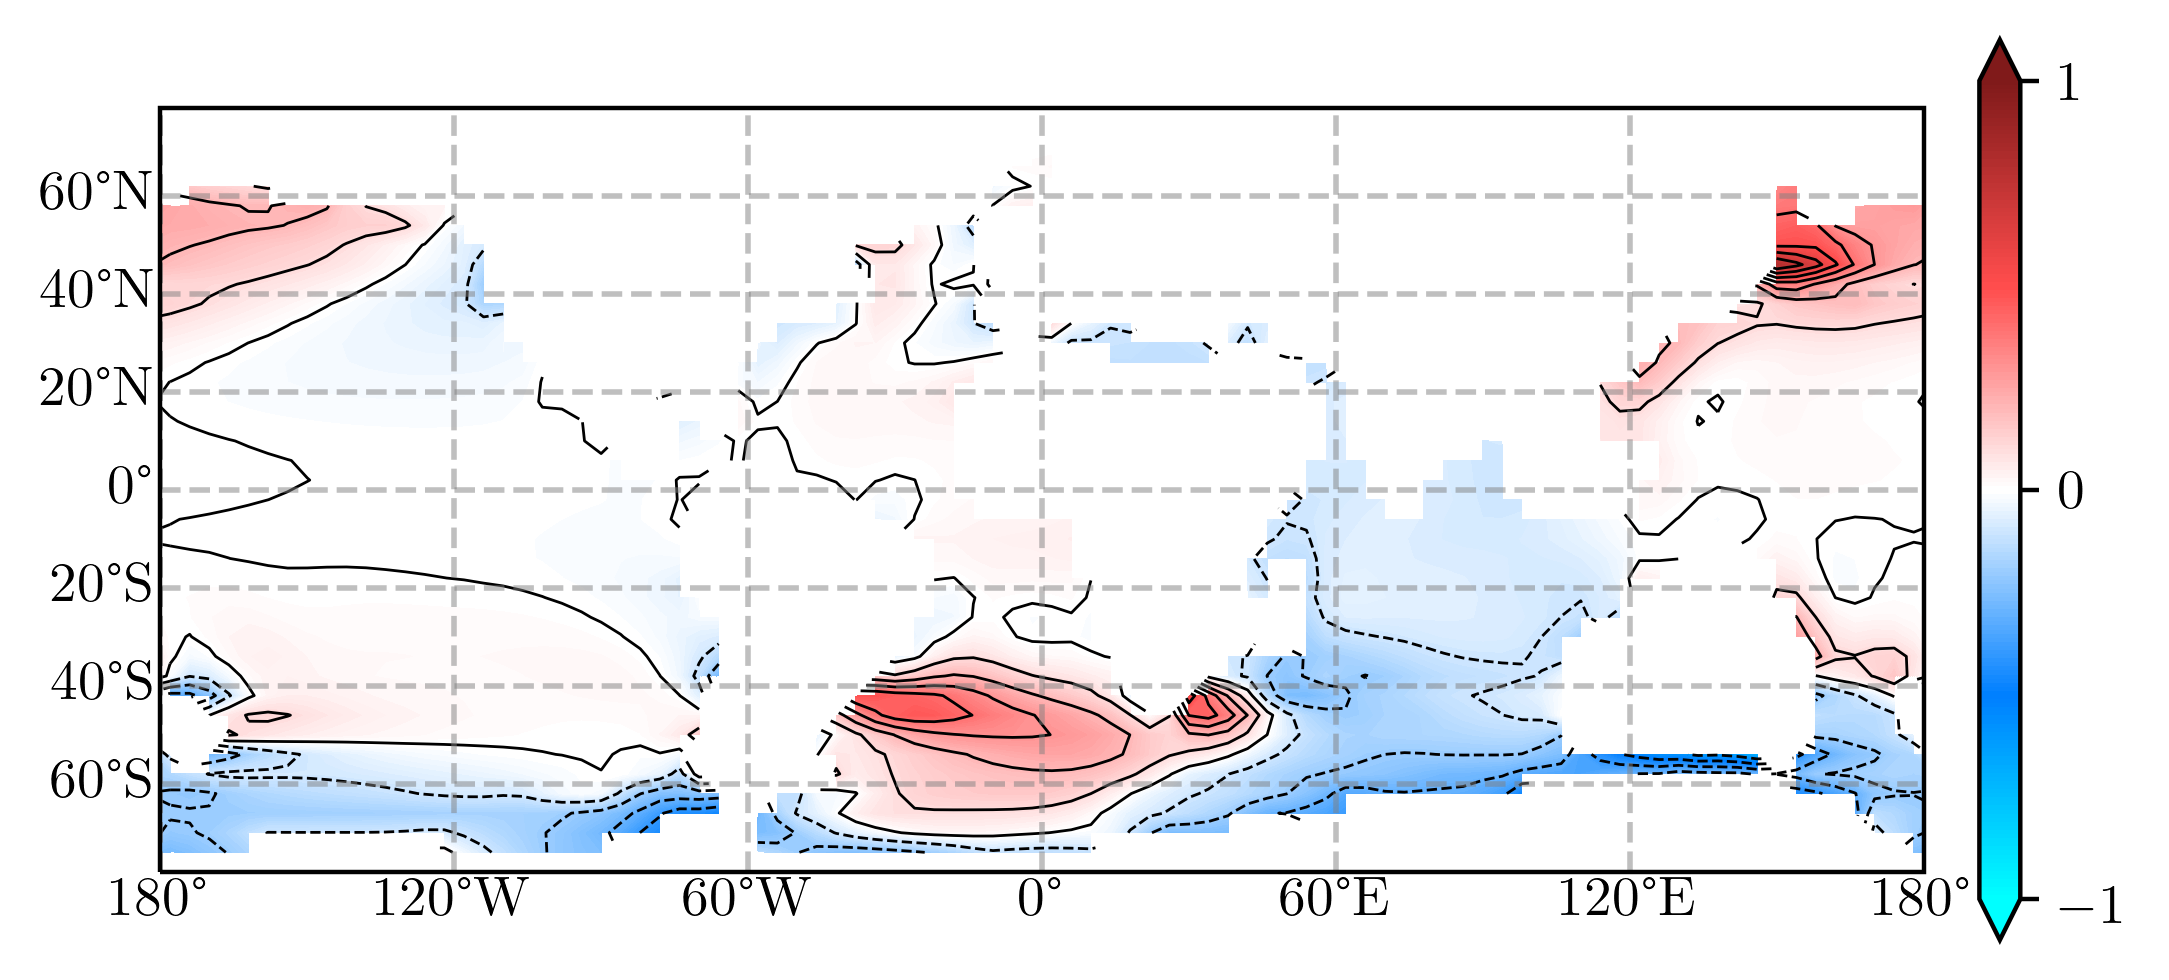
\includegraphics[width=\linewidth]{salt_35_20.png}
	\caption{SSS}
	\label{fig:salt3520cooling}
\end{figure}
\begin{figure}[H]
	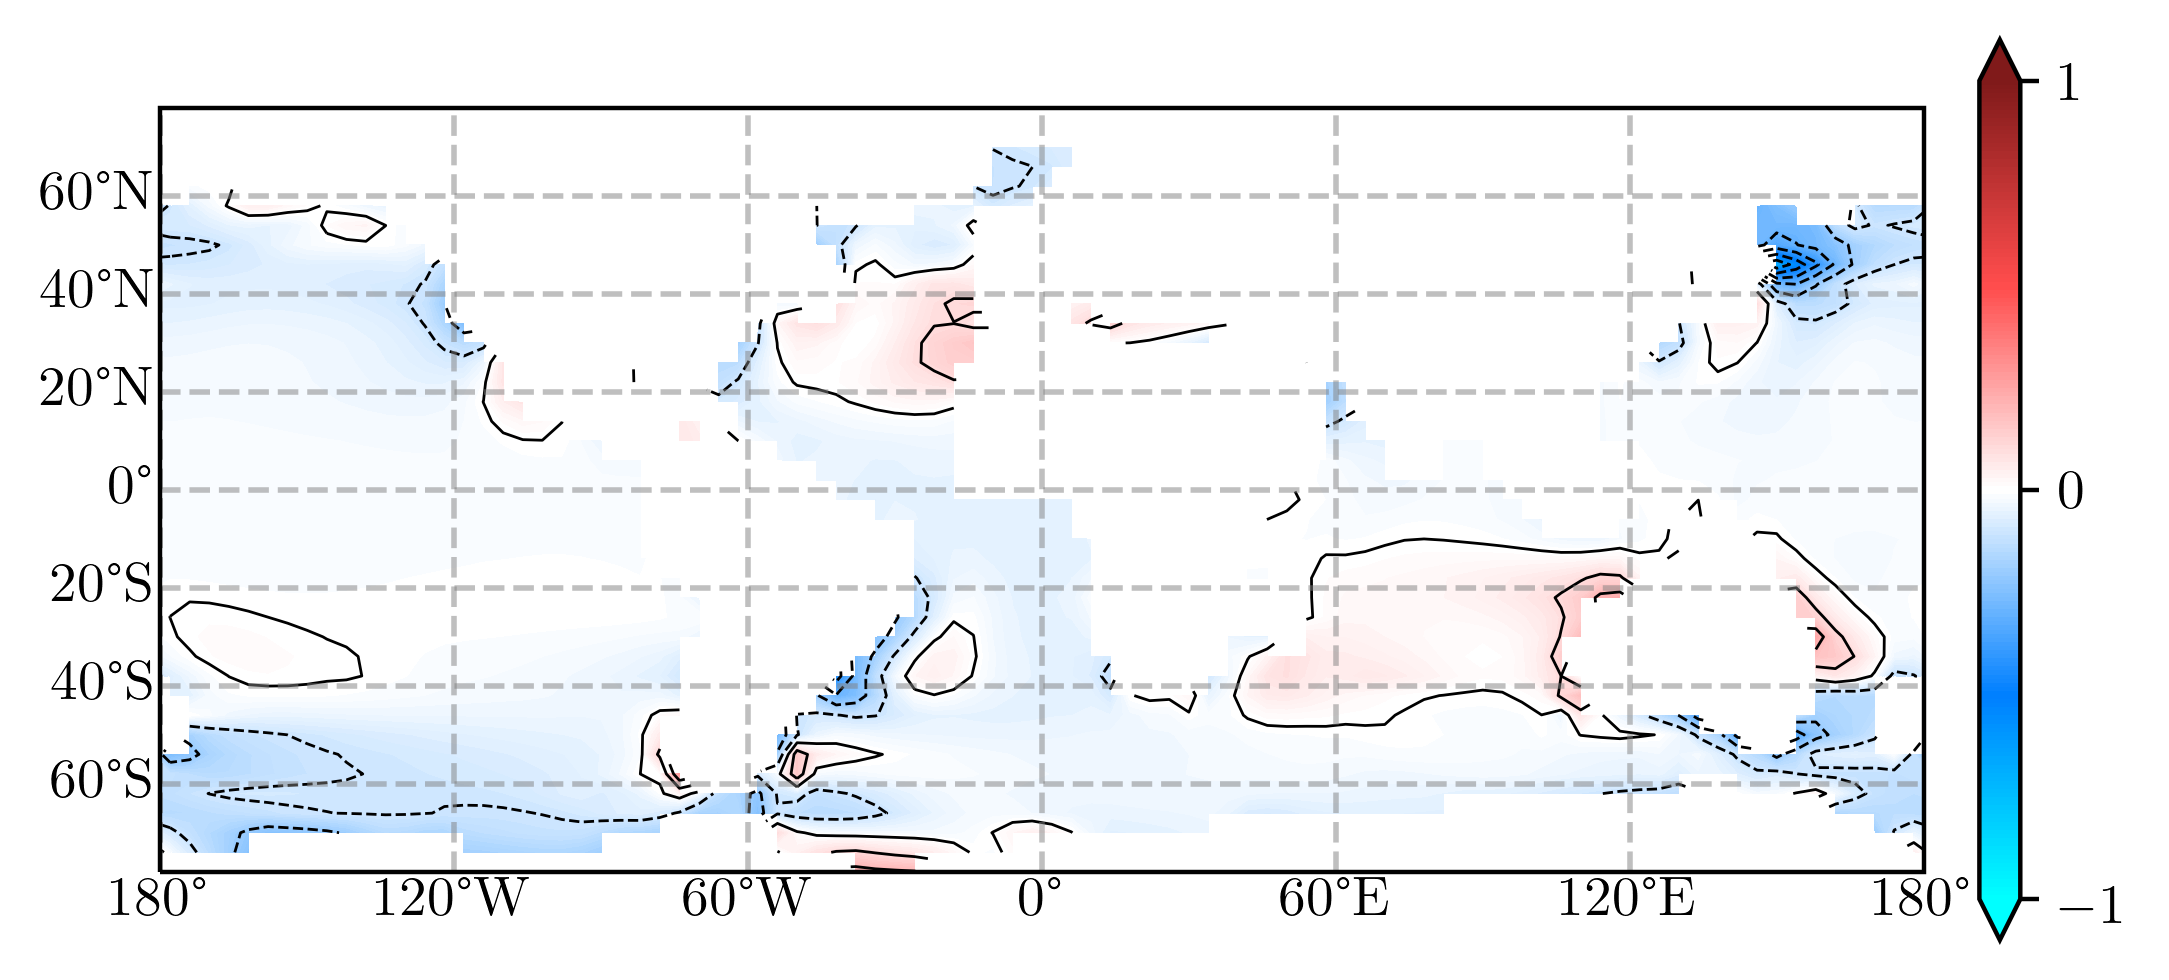
\includegraphics[width=\linewidth]{salt_20_10.png}
	\caption{SSS}
	\label{fig:salt2010cooling}
\end{figure}

